
\subsection{Data}

We curate and synthesize a large-scale, multi-domain corpus of post-training data spanning Agentic Software Engineering, Complex Tool Use, and Agentic Cowork. By systematically expanding its task diversity and difficulty frontier, we aim to push compact models toward performance ceiling and probe the limits of capability that can be unlocked through high-quality, scalable supervision.

\subsubsection{Agentic Software Engineering: Repository-to-Trajectory Synthesis.}\label{agent-coding}

\begin{figure*}[t!]
    \centering
    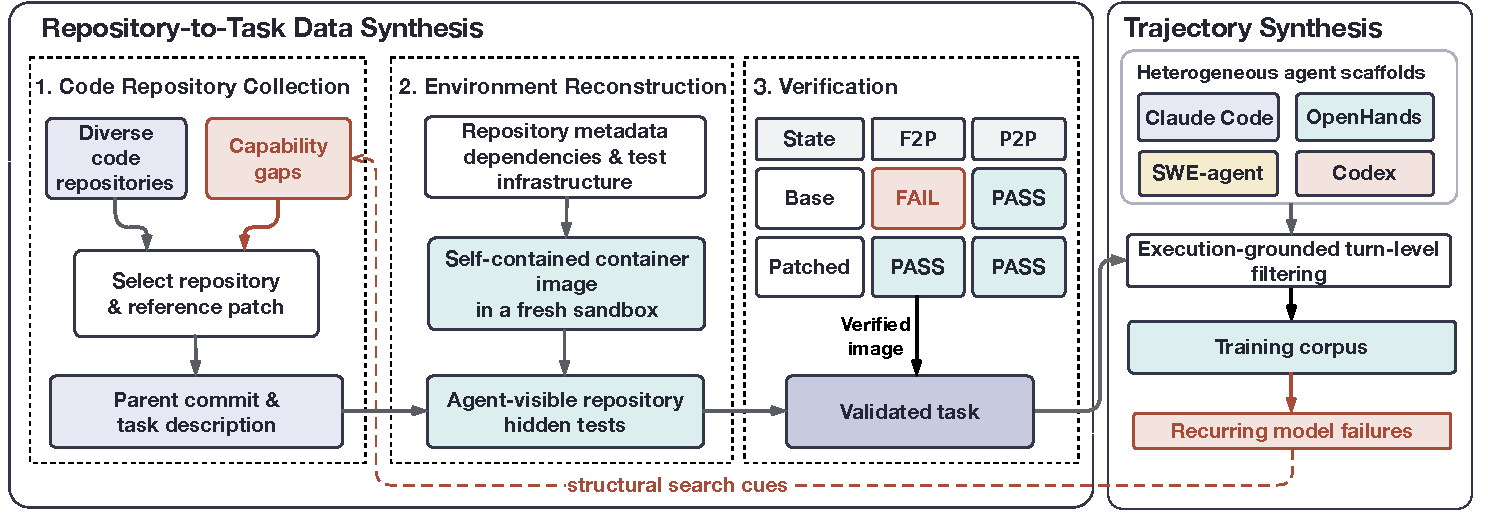
\includegraphics[width=1\textwidth]{figures/agent-data.pdf}
    \caption{Agentic Software Engineering Data Synthesis Pipeline.}
    \label{fig:error2task_pipeline}
\end{figure*}

Unlike single-turn code generation, real-world agentic coding demands that models navigate complex repositories, infer intent from ambiguous specifications, localize defect paths, apply coordinated multi-file patches, and verify correctness via closed-loop execution. To construct high-quality trajectory supervision at scale, we establish a repository-level data synthesis pipeline. This system transforms historical GitHub development activities into executable tasks backed by automated environments, while leveraging model failure feedback to co-evolve task distribution alongside agent capabilities. The resulting repository-to-task data synthesis process is illustrated in Figure~\ref{fig:error2task_pipeline}.

\paratitle{Capability-Guided Code Repository Collection.}
To ensure the diversity and scale of our data, we first collect code repositories spanning programming languages, project scales, and application domains, from which we construct well-scoped software-engineering tasks with executable verification. 
To further identify repositories with the greatest potential to improve model capabilities, we run our model on a small set of seed training tasks, analyze and categorize its failure modes, and use the resulting capability gaps to guide repository and patch selection. 
This process preserves diversity across repositories and problem settings while improving coverage of capability areas in which the model exhibits systematic weaknesses.

\paratitle{Executable Environment Reconstruction and Task Synthesis.}
Once a repository is prepared and the patch is selected, we reconstruct the execution environment by analyzing repository metadata, dependency specifications, and test infrastructure. We then build a self-contained container image from the parent commit in an isolated sandbox.
Tasks are synthesized based on the selected patches, while the patches themselves and task-specific grading tests are withheld from the repository exposed to the agent.
Hidden tests are injected only during evaluation.


\paratitle{Verification and Closed-Loop Task Evolution.}
Before trajectory synthesis, we validate each task using an executable verifier constructed from the original source and test changes. 
Fail-to-pass tests confirm that the target behavior is absent in the base repository and restored by the reference patch, while pass-to-pass tests protect existing functionality from regression. 
We also audit whether the task description, hidden tests, and reference patch express a consistent behavioral contract, revising recoverable tasks and discarding broken, flaky, or underspecified ones. 
During routine inference and training, recurring model failures are automatically collected and converted into structural search cues for subsequent repository mining. 
This closed-loop mechanism expands the task space to systematically concentrate on weaknesses detected during the model’s own evolution.



\paratitle{Trajectory Synthesis across Diverse Scaffolds.}
To prevent model over-fitting to specific prompt templates or tool-use conventions, we deploy multiple heterogeneous agent scaffolds within our containerized sandbox, including Claude Code, OpenHands, SWE-agent, and specialized Codex-based drivers.
Given the same repository state and fail-to-pass verification tasks, each agent independently explores and resolves problems in parallel. 
Their distinct system prompts, context compression policies, and editing interfaces induce diverse solution strategies (e.g., broad exploratory search vs. localized pinpoint editing). 
Aggregating these complementary trajectories yields a training corpus that emphasizes scaffold-invariant reasoning and repair strategies, rather than scaffold-specific interaction patterns, thereby improving generalization to unseen agent interfaces and tool schemas.


\paragraph{Execution-Grounded Turn-Level Filtering.}
To ensure data quality, we retain only trajectories whose resulting patches pass the designated target and regression tests. 
We further conduct a turn-level filtering for incorrect tool calls, non-terminating loops, redundant actions, and context truncations, prioritizing concise trajectories while preserving essential debugging and recovery steps. 
Finally, all trajectories are normalized into a unified multi-turn schema comprising observed assistant messages, tool calls, and environment feedback.



\subsubsection{Tool Use: Scaling Trajectory Synthesis with Hybrid Real-Simulated Environments.} 

% Tool use underpins agentic competence. 
We collect and synthesize a large corpus of high-quality tool-use trajectories.
Building upon the data-synthesis pipeline developed for Nanbeige4.1~\cite{yang2025toolmind}, we further scale the diversity and complexity of tool-use tasks by constructing hybrid environments that integrate real-world APIs, executable tool interfaces, and model-simulated environmental components.
The resulting framework comprises four components as illustrated in Figure~\ref{fig:mcp}: tool specification collection, executable environment synthesis, task synthesis, and a difficulty taxonomy that supports automated labeling and adaptive evolution.


\begin{figure*}[t!]
	\centering
	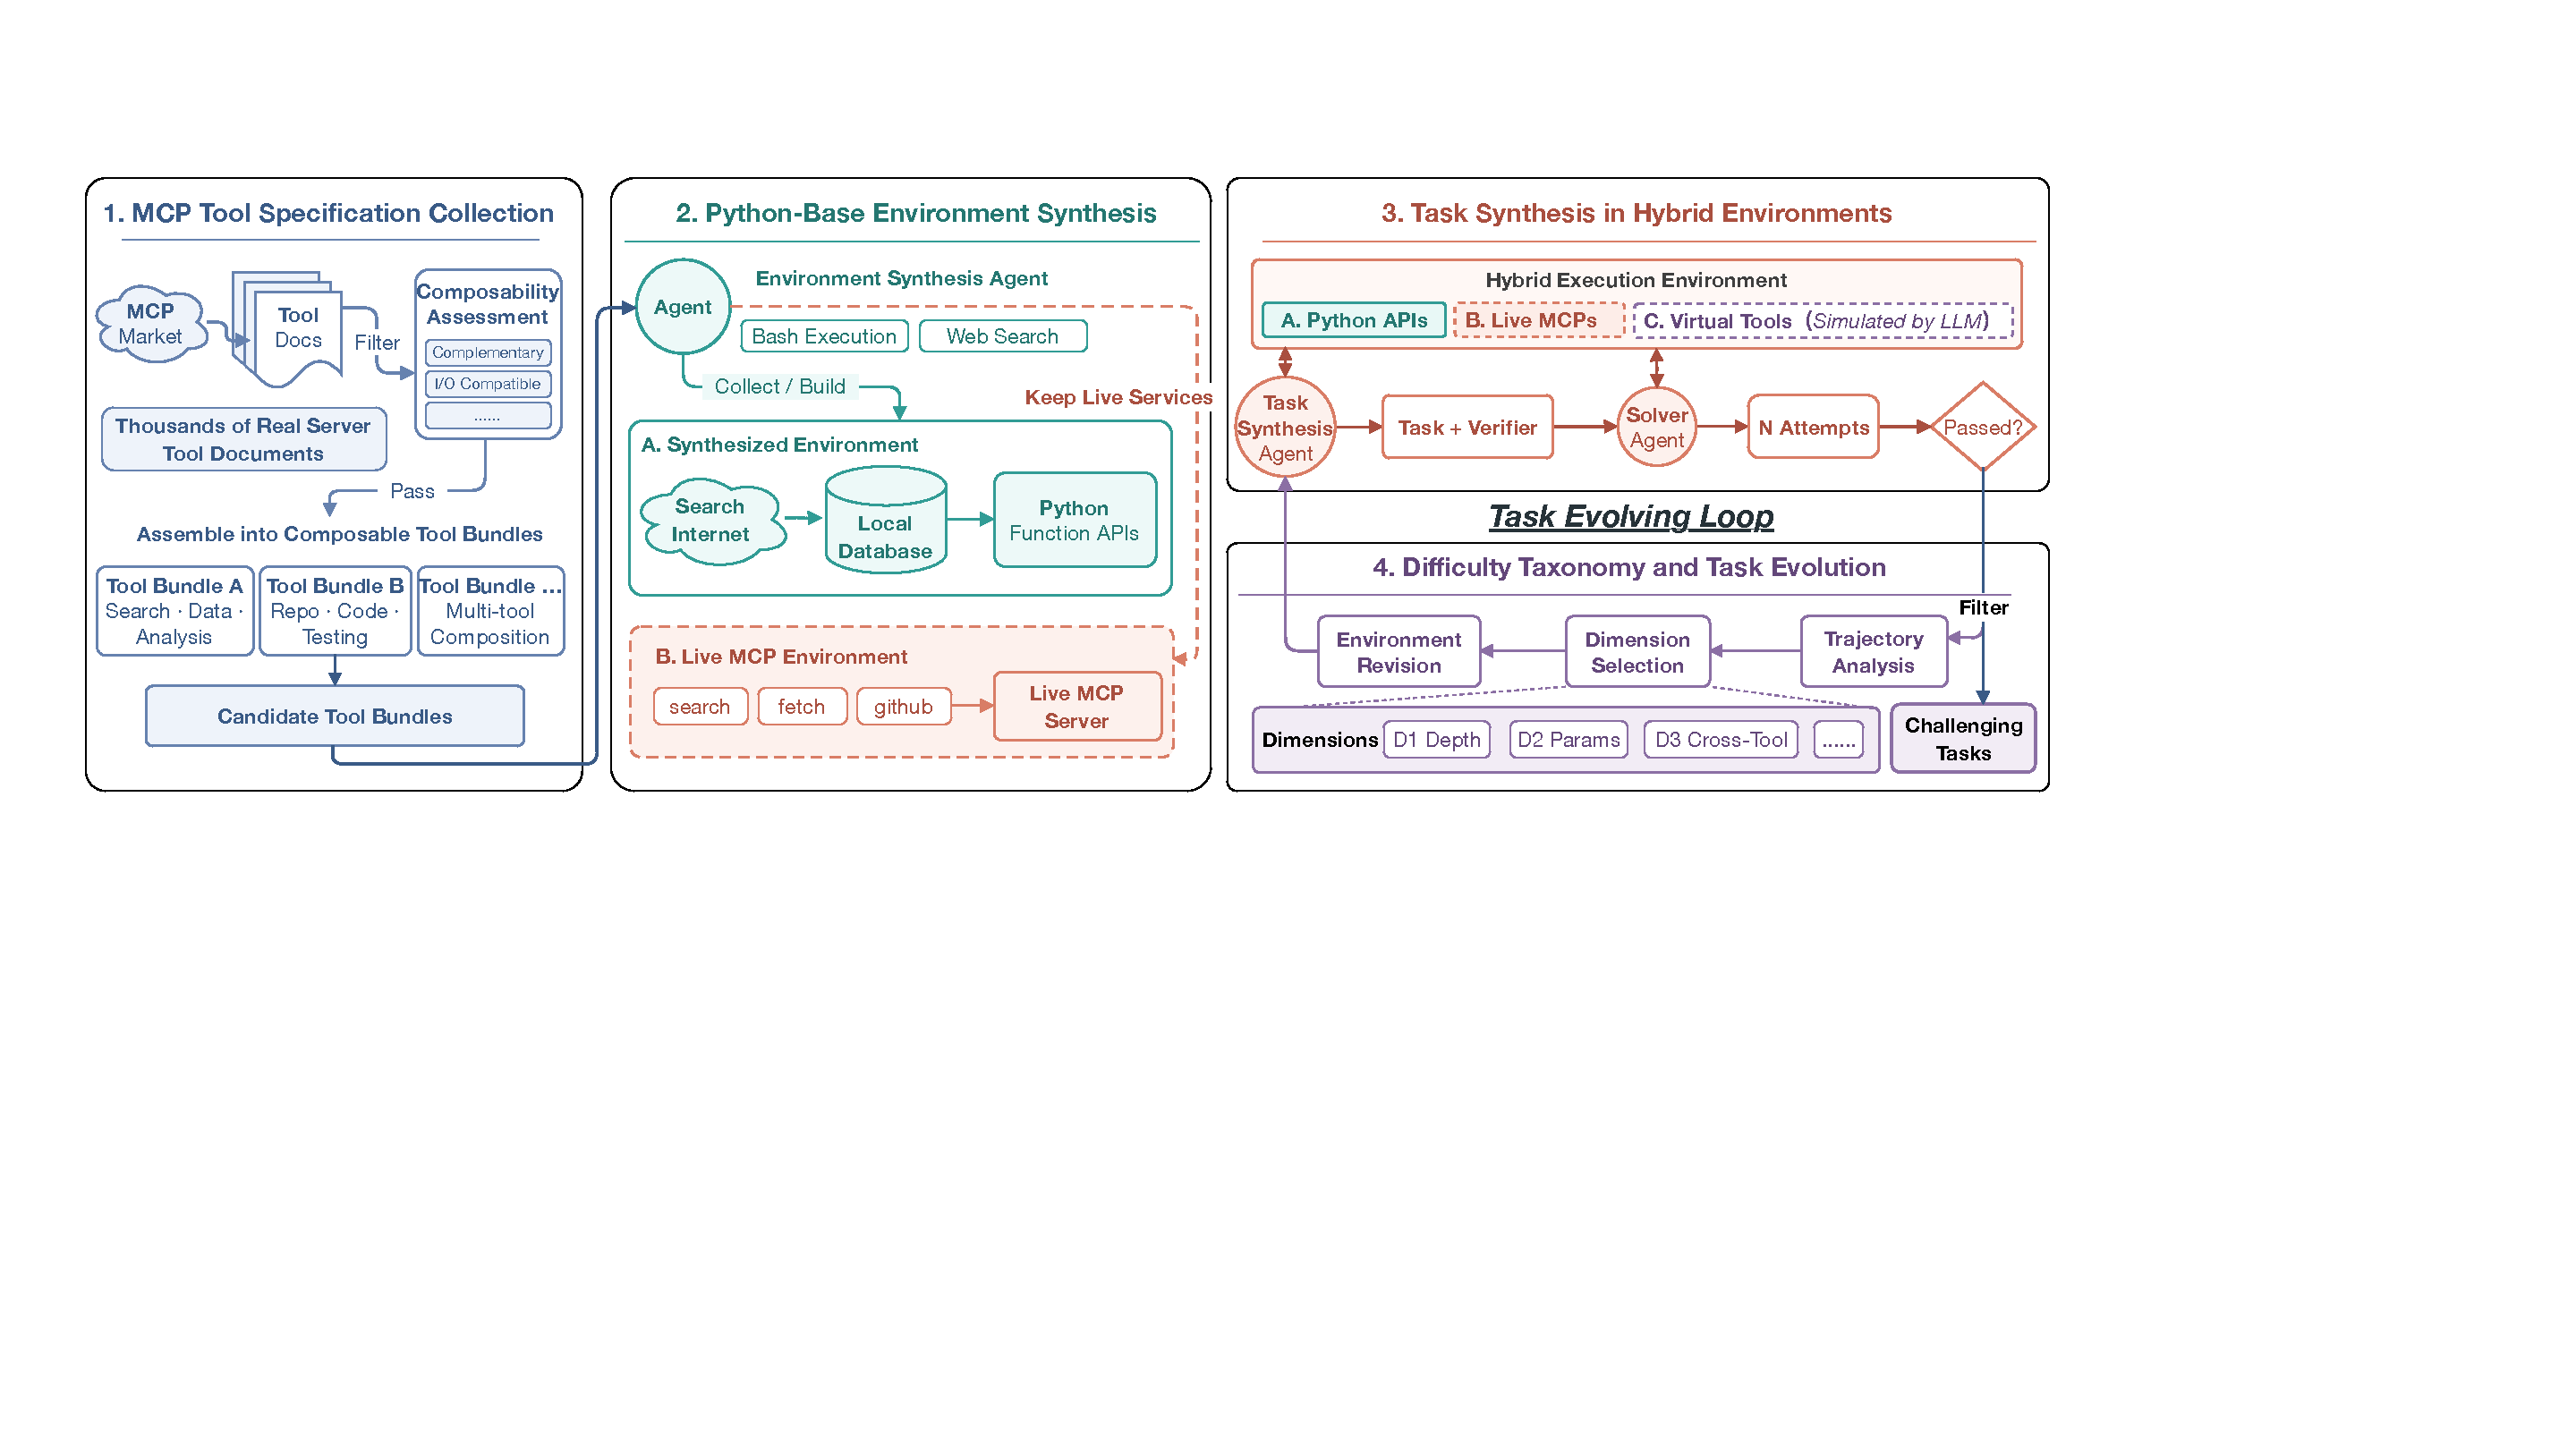
\includegraphics[width=1\textwidth]{./figures/mcp-black.pdf}
	\caption{\textcolor{black}{Tool Use Data Synthesis Pipeline.
 }}
	\label{fig:mcp}
\end{figure*}

\paratitle{MCP Tool Specification Collection.}
We collect thousands of tool specification documents for real-world MCP servers from MCP marketplaces. For each, we assess its composability---that is, whether it can be orchestrated with other tools to support complex, multi-step tool-use scenarios. 
Then, tools with sufficient compositional potential are grouped into bundles that serve as the foundation for downstream task construction.


\paratitle{Python-Based Executable Environment Synthesis.}
For each tool-documentation bundle, an environment-synthesis agent equipped with web-search and Bash-execution capabilities automatically acquires relevant real-world data from the Internet and persists it in a local database. It then uses Python to reconstruct each tool as a callable function interface, thereby creating a self-contained execution environment that combines real data with a complete tool suite.


\paratitle{Task Synthesis in Hybrid Environments.}
Beyond Python-based executable environments, we retain live MCP services for tools such as web search, web scraping, and code-repository access, whose dynamic and time-sensitive outputs cannot be faithfully captured by static databases. For tools that depend on extensive runtime environments and cannot be readily reproduced in Python, we instead use a model to simulate their behavior and outputs.
Accordingly, our synthesis pipeline integrates three complementary environment types: (1) live online MCP services, (2) local tools implemented in Python, and (3) model-simulated virtual tools. This design supports both customized tool-use scenarios with complex data dependencies and general-purpose tool use requiring real network interaction, balancing environmental diversity with ecological realism.


\paratitle{Difficulty Taxonomy and Adaptive Task Evolution.}
To ensure that synthesized tasks attain sufficient difficulty and complexity, we predefine a difficulty taxonomy that systematically characterizes tasks along multiple dimensions, such as tool-use chain depth, information-retrieval difficulty, and parameter-inference complexity. Conditioned on the current environment, a task-synthesis agent with access to Bash execution generates natural-language task specifications together with Python verification functions for programmatic correctness evaluation.
After synthesis, a solver agent attempts each task multiple times. Trajectories from reliably solved tasks are fed back to the task-synthesis agent to identify the model's capability frontier and selectively evolve tasks by increasing difficulty along the relevant dimensions, thereby establishing an iterative closed-loop process.


\paratitle{Rapid Validation Construction.}
\label{sec:rapid_validation}
In parallel, we construct a compact held-out task suite for rapid validation during development. The suite covers representative tool bundles, hybrid environment types, and difficulty levels, while remaining disjoint from the training data. It enables fast and reproducible assessment of whether successive data-synthesis and reinforcement-learning iterations improve tool-use performance before full-scale evaluation.



\subsubsection{Agentic Cowork: Scaling Complex Office Tasks through Artifact-Centric Curation.} 


Beyond foundational tool use, agents must handle specialized office workflows involving reports, slide decks, spreadsheets, and other artifacts—capabilities central to knowledge-worker productivity. 
To equip foundation models with this agentic cowork capabilities, we develop an artifact-centric curation pipeline that synthesizes, evolves, and recycles task artifacts to scale diverse and complex real-world office workflows. 
In detail, the pipeline comprises artifact repository construction, vector-similarity-based domain clustering, task synthesis, trajectory synthesis, and closed-loop artifact reuse, as illustrated in Figure~\ref{fig:agentic_cowork_pipeline}.


\begin{figure*}[t!]
	\centering
	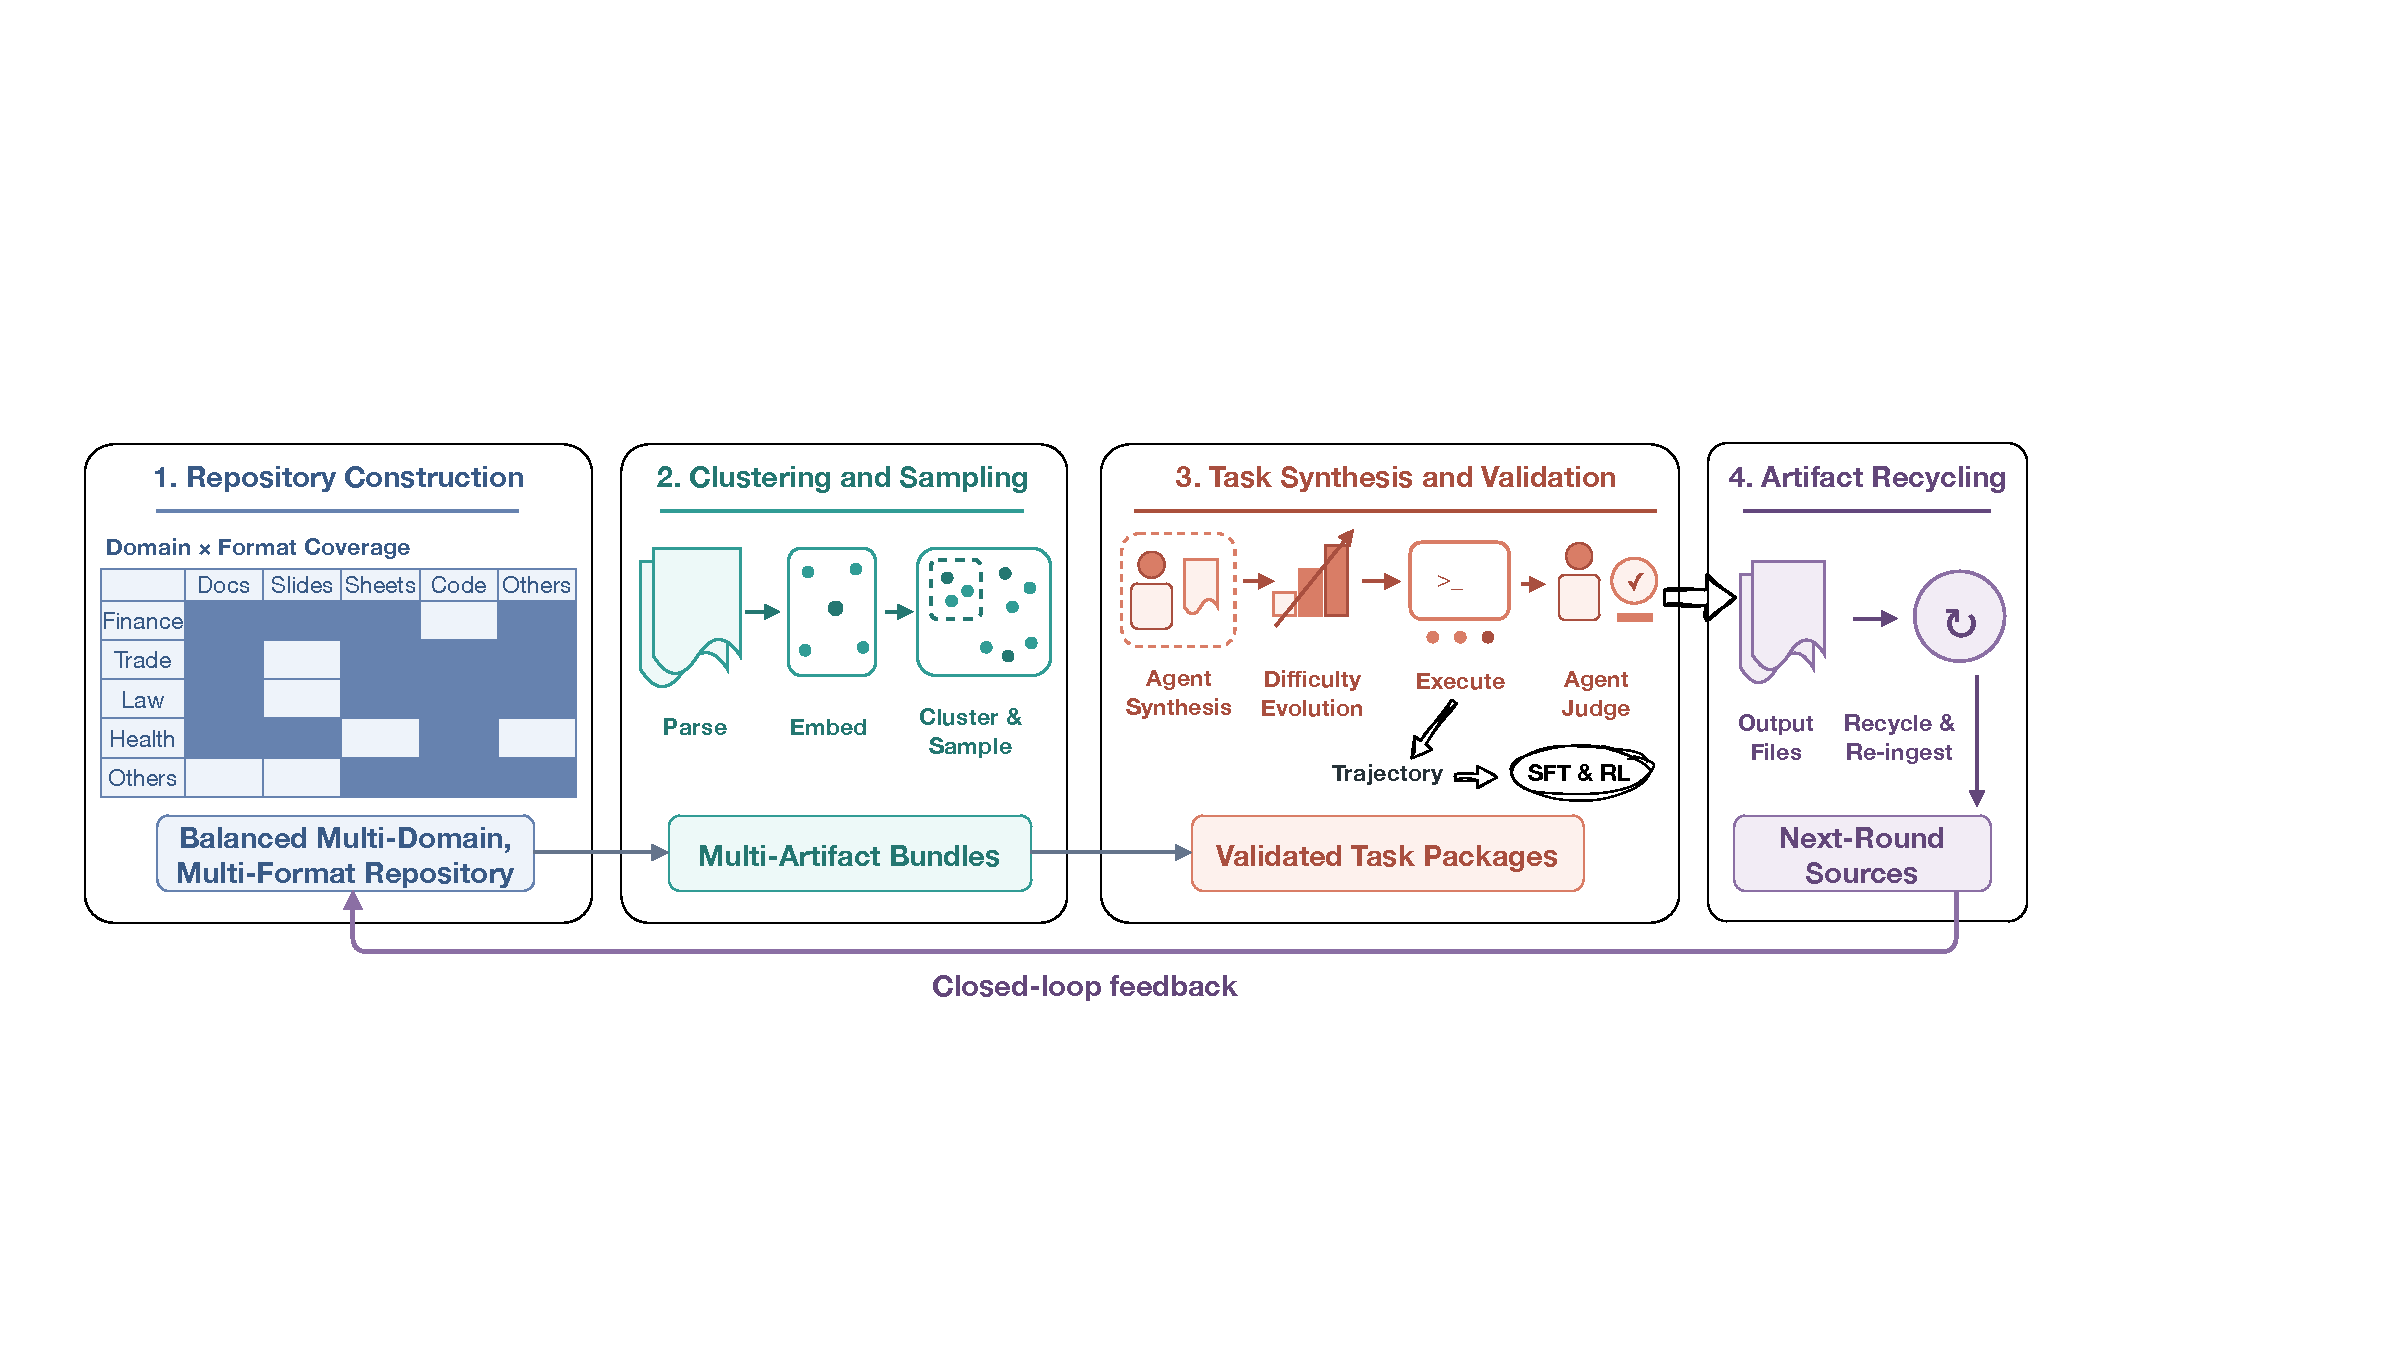
\includegraphics[width=1\textwidth]{./figures/cowork-black.pdf}
	\caption{\textcolor{black}{Agentic Cowork Data Synthesis Pipeline.
 }}
	\label{fig:agentic_cowork_pipeline}
\end{figure*}


\paratitle{Artifact Repository Construction.}
We construct a balanced artifact repository by collecting materials from diverse professional domains, including finance, trade, law, healthcare, and others. The repository covers heterogeneous formats, such as reports, slide decks, spreadsheets, PDFs, emails, and others, while calibrating their relative proportions to achieve broad and realistic coverage.

\paratitle{Embedding-Based Domain Clustering.}
We parse and normalize the collected artifacts into structured representations, encode them into a shared embedding space, and cluster them according to semantic and domain similarity. We further group and sample artifacts within each cluster to construct coherent yet diverse multi-artifact bundles for downstream task synthesis.

\paratitle{Task, Rubric, and Trajectory Synthesis.}
A task-synthesis agent interactively explores and manipulates selected artifact bundles within a sandboxed workspace to synthesize office tasks and their evaluation rubrics. We assign difficulty tiers and iteratively evolve tasks along multiple dimensions, including cross-artifact dependencies, tool-use requirements, workflow length, constraints, and verification demands. Open-source models subsequently execute the resulting tasks to generate tool-use trajectories and deliverable artifacts. An independent judge agent then evaluates the fidelity of each deliverable to the task specification, the consistency of the associated rubric, and the overall quality of the execution trace, retaining only high-quality samples for subsequent synthesis rounds.


\paratitle{Closed-Loop Artifact Recycling.}
Validated deliverables are re-ingested into the artifact repository as source materials for subsequent synthesis rounds. This closed-loop process progressively expands the task distribution, enabling the generation of increasingly diverse and complex office workflows.


